% Methedology: 2,000 words

\chapter{Methodology}

The primary objective of our study is to develop an AI model using the technique of transfer-learning, to automatically predict RUST scores from an input radiograph. In this chapter, we will first discuss our experiment design, contextualising the choices we make in our methodology and evaluation. Next, we will briefly summarise the datasets used in the study, before proceeding to the main methodology (protocols) itself. Afterwards, the evaluation and endpoints will be presented, as well as a discussion on patient privacy and ethical considerations.

\section{Model Design}

Transfer learning is a technique which uses a model trained upon a larger dataset first, before being applied to a smaller, task-specific dataset. Assuming our task-specific dataset (in our case, the RUST data from METRC) is fixed, the performance of our transfer-learning model is determined by the following factors:

\begin{enumerate}
    \item The architecture of the original model.
    \item The initial, large dataset that the original model is trained on.
\end{enumerate}

\noindent
Hence, in the context of our study design, we must first choose (or create) a model architecture, and select an initial large dataset to train our model on. Only then are we able to apply the transfer learning procedure (e.g. freeze model weights, add new classifier, fine tuning, etc) upon our task-specific dataset.

\subsection{Model Architecture Choices}

The first decision that we must make in our experiment design is the choice of model architecture.
According to a literature survey by Litjens, Kooi, Bejnordi et al., convolutional neural networks (CNNs) are the most common deep learning architecture deployed for medical image analysis, vastly outnumbering alternative methods such as Stacked Autoencoders (SAE), or Recurrent Neural Networks (RNNs) \autocite[77]{cnn-most-common}.
This is expected, as CNNs exhibit strong performance with image classification tasks, and as our project is an image classification task (albeit with radiographs), we will be using a CNN.

The choice now remains to either design our own CNN from scratch, or use an existing CNN architecture.
Although designing a CNN \emph{ab initio} allows the possibility of further experimentation and potentially finer-grained control, such a \emph{de novo} model is difficult to assess holistically: there would be no prior work in literature to serve as a basis for comparison.
In contrast, if we use a well-documented, existing CNN as our transfer-learning foundation, we may compare the performance of our implementation against other instances of the same model architecture used for transfer-learning in different domains.
% The commensurability of a standard model for comparison is important: in a 2022 review of transfer learning techniques in medical image analysis, Kora, Ooi, Faust et al. found that only 13\% of prior studies compared their results with other models \autocite[94]{kora2022}. 

Thus, we will be using the InceptionV3 model, a convolutional neural network developed by Szegedy, Vanhoucke, Ioffe, et al. from Google \autocite{inceptionv3}. Our choice of InceptionV3 is based upon a 2022 literature review of transfer-learning models for the domain of medical image analysis. According to Kora, Ooi, Faust et al., CNNs with a broad (as opposed to deep) network topology perform well in transfer-learning tasks \autocite{kora2022}, with models like InceptionV3 outperforming more parameterized models like AlexNet \autocite{alexnet}. Indeed out of the 54 studies included in the review, Inception-style models both the most common (14 out of 54) and among the highest-performing. \autocite{kora2022}

\subsection{\enquote*{Top-Classifier} Choices}

\emph{This subsection is unavailable in this version of the document.}

\subsection{Model Optimizer Choices}

Finally, the last architectural decision we must make in our model design, is the choice of an optimizer. We have two possible approaches: we may either select an optimizer from \emph{a priori} principles, or consider the selection of an optimizer to be a hyperparameter, and benchmark a variety of optimizers with our model on the data-set. Because we are already evaluating two variants of InceptionV3, the additional task of iterating through different optimizers will be infeasible given the time and compute constraints of the project.

Hence, our choice of an optimizer is determined by a review of available benchmarks and literature. The study and benchmarking of deep learning optimizers is a fairly recent field, initiated by the development of robust, reproducible benchmarks. Projects like Schneider, Balles, et Hennig's \emph{DeepOBS: A Deep Learning Optimizer Benchmark Suite} allowed researchers to evaluate optimizers against an assay of realistic optimization problems, simulating common deep learning tasks and neural network architectures. \autocite{deepobs} The availability of reproducible benchmarks allowed the first large-scale empirical experiments to be conducted on optimizer performance, culminating in Schmidt, Schneider, et Hennig's 2021 paper in optimizer benchmarking. \autocite{crowdedvalley} In an evaluation of 15 popular optimizers\footnote{AMSBound, AMSGrad, AdaBelief, AdaBound, AdaDelta, Adam, LookaheadMomentum, LookaheadRAdam, Momentum, NAG, NAdam, RAdam, RMSProp, and SGD, respectively. The full list of results are available in their supplementary appendix.} across a total of more than 50,000 epochs of training, significant data on optimizer performance was gathered.

Of the eight optimization problem assays in the benchmark suite, our task of radiographic image classification is bears closest resemblance to the CIFAR-10 benchmark: a CNN-based image classification task. According to the latest results available on the paper's website\footnote{\url{https://deepobs.github.io/leaderboardP4.html}}, the ADAM optimizer has a slight accuracy improvement over Momentum and SDG. However, the differences are so small that the author mentions: \blockcquote[2]{crowdedvalley}{
    \ldots\ a practitioner with a new deep learning task can expect to do about equally well by taking almost \emph{any method} from our benchmark and tuning it, as they would by investing the same computational resources into running a set of optimizers with their default settings and picking the winner.
}

\noindent
Therefore, we will select the ADAM optimizer, and spend time on fine-tuning the model and hyperparameter choices, instead of devoting further resources to selecting an optimizer.

\subsection{Pre-Training Dataset Choices}

Now that we decided our model architecture, the next step is to select the initial, or pre-training dataset, that is used to train our model.

\subsubsection{ImageNet Dataset}
Originally, InceptionV3 was trained on the ImageNet dataset: a general-purpose collection of more than 14 million everyday images. \autocite{imagenet} The overwhelming size of the ImageNet dataset serves as a robust foundation for the InceptionV3 model, which exhibits strong performance in classification tasks upon it. However, the statistical characteristics of data in ImageNet is quite different from data in a typical radiography dataset. Hence, it remains a valid research question to ask whether a InceptionV3 model trained on a smaller, but more domain-specific dataset will exhibit better performance when applied to our transfer-learning task.

\subsubsection{RadImageNet Dataset}
Thus, we will also investigate RadImageNet, a collection of 5 million medical images composing of radiographic (CT), MRI, and ultrasound images. \autocite{radimagenet} As an open radiologic dataset developed specifically for transfer learning applications, a base model trained on RadImageNet may exhibit better performance on our radiography data, as the original network is trained upon images in a similar domain. However, the advantages of a similar domain is moderated by the corresponding smaller dataset size (5 million versus ImageNet's 14 million).

Therefore, in this project we will evaluate the use of a InceptionV3 model trained both on the ImageNet dataset, as well as the RadImageNet dataset as the base model for transfer learning. By comparing the performance of both models, we will be able to select the best-performing one for further development and refinement. Additionally, the additional data point afforded by a second model allows greater context for our evaluation: according to Kora et al., only 13\% of transfer-learning studies benchmarked their model performance against a second model. \autocite[94]{kora2022} By choosing to evaluate two models from the very start of our project's design, we get to avoid this scientific blind-spot: and hopefully achieve a better result overall.

\section{Data Egress and Preprocessing}

Now that we have defined the design of our experiment, we must define the pre-processing and data egress requirements.
Our study data consists of anteroposterior and lateral view radiographs, as well as their corresponding RUST scores. This data is provided in a collaboration with METRC, Johns Hopkins University, through their archive of past and on-going studies. \autocites{RetroDEFECT2022}{OUTLET2021}{PAIN2017}{PACS2022} The data is held within REDCap: an electronic data and clinical trials database. \autocite{redcap} Because the data is held across multiple clinical trials and within multiple instruments, egressing data out of REDCap and pre-processing it into a useable form is a non-trivial software engineering task.

\begin{table}[H]
    \centering
    \begin{tabularx}{\textwidth}{@{}lXr@{}}
    \toprule
    \textbf{Dataset}     & \textbf{Name} & \textbf{Samples} \\ \midrule
    \autocite{RetroDEFECT2022} \textsc{RetroDEFECT} & \emph{Retrospective Study of the Treatment of Long Bone Defects}    & $741$             \\
    \autocite{OUTLET2021} \textsc{Outlet}      & \emph{Outcomes Following Severe Distal Tibia, Ankle and/or Foot Trauma}     & $707$             \\
    \autocite{PAIN2017} \textsc{Pain}        & \emph{Pain Management \& Long Term Outcomes Following High Energy Orthopedic Trauma}      & $370$             \\
    \autocite{PACS2022} \textsc{Pacs}        & \emph{Predicting Acute Compartment Syndrome using Optimized Clinical Assessment}    & $195$             \\ \midrule
    Sum         &      & $2,013$            \\ \bottomrule
    \end{tabularx}%
    \caption{Sources of Radiographic Data with RUST labels in REDCap}\label{tab:datasets}
\end{table}

\subsection{Validate Radiography Data with Branch-Parser}

The first challenge that we face in the data egress process, is finding RUST-radiography pairings that are valid for inclusion in our dataset. A small subset of radiographs do not possess valid RUST scores: either because they were uninterpretable due to hardware occlusion (e.g. presence of a titanium orthopaedic fixture), or because the radiograph was not taken for the purpose of assessing fracture healing. In order to validate the radiography data, a Python package called redcap-branch-parser was developed to parse the conditional logic contained within REDCap patient records. \autocite{redcap-branch-parser} The development of this package took up a non-trivial amount of early project work.

Once valid RUST-radiograph pairs were identified, the study data was egressed out of REDCap using a set of ad-hoc Jupyter Notebooks and the PyCap API package. \autocite{pycap}

\subsection{Automated de-skewing with ImageMagick}
Following the egress of radiography data, the radiography image files were automatically de-skewed using ImageMagic. At this point, data-preprocessing is complete, as data augmentation will be performed dynamically via layers within Keras.

\section{Data Augmentation Strategy}

Because we have a small dataset, a robust data augmentation strategy is needed to combat overfitting. In order to develop our data augmentation strategy, we followed suggestions from Bejani et Ghatee's \emph{systematic review on overfitting control in shallow and deep neural networks} \autocite{overfitting-prevention}. We may categorise data augmentation strategies to three broad families of methods: \autocite{augmentation-strategies}

\begin{enumerate}
    \item \textbf{Geometric Methods:} rotation, cropping, flipping.
    \item \textbf{Photometric Methods:} noise, color-shifting, edge modification.
    \item \textbf{\enquote*{Complex} Methods:} generating artificial data using GANs, style transfer.
\end{enumerate}

\noindent
Of the three, \enquote*{complex} data augmentation methods such as generating artificial data points is inappropriate for our use case, as it will compromise the evidence-based labelling of our dataset. Hence, we may recourse to either geometric methods, or photometric methods. Originally, our intuition was that photometric data augmentation methods would be of limited applicability to radiographs, which are entirely greyscale. Upon further investigation, it turns out that when evaluated individually, the most effective data augmentation strategy is cropping, followed by rotation. \autocite{benchmark}

Hence, in order to avoid potentially compromising our small dataset with too much noise, our data augmentation strategy will be restricted to geometric methods such as rotation, cropping, and flipping.

\clearpage

\section{Protocols}

Now that we have finished discussing the model design, data egress, and augmentation, it is time to define the study protocols. The experimental portion of this study will consist of three protocols:

\begin{enumerate}
    \item Protocol   I: A \enquote*{naive} CNN without transfer-learning, for use as a baseline.
    \item Protocol  II: Transfer-learning w/ InceptionV3 trained on ImageNet.
    \item Protocol III: Transfer-learning w/ InceptionV3 trained on RadImageNet.
\end{enumerate}

\noindent
All protocols will utilise the same data augmentation pipeline.

\begin{figure}[H]
    \centering
    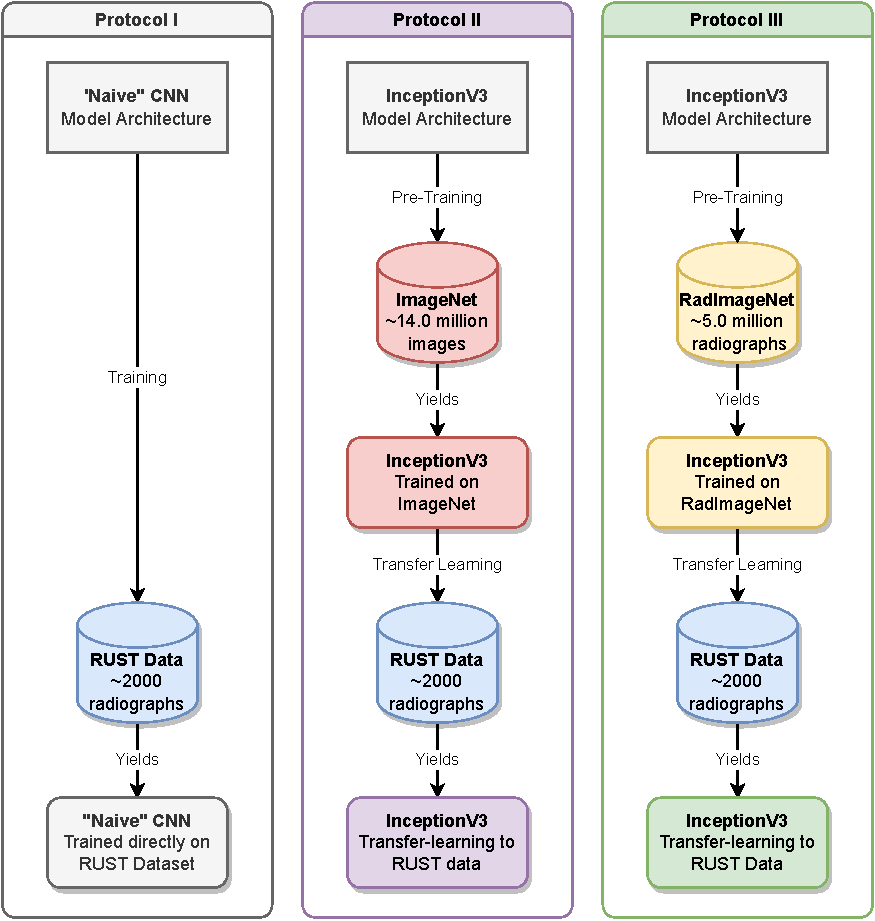
\includegraphics[
        page=1,
        width=\textwidth,
        angle=0,
        right
    ]{media/protocol-diagram.pdf}
    \caption{Overview illustrating the three model development protocols.}
    \label{fig:protocols}
\end{figure}

\subsection{Protocol I: \enquote*{Naive} CNN Baseline}

In protocol I, we will develop a \enquote*{naive} CNN without the use of transfer learning, that is trained directly on the RUST dataset. This model will serve as a performance baseline to benchmark our transfer-learning models against.

\subsubsection{\enquote*{Naive} CNN Architecture}

\emph{This subsection is unavailable in this version of the document.}

\subsection{Protocol II: InceptionV3 with ImageNet}

In protocol II, we will use InceptionV3 trained on the ImageNet dataset as a base model for transfer-learning.

\noindent
\emph{This is an outline. More information will be added later.}

\begin{enumerate}
    \item Instantiate base model with pre-trained weights.
    \item Freeze weights in base model. Remove output (classifier) from base model.
    \item Create a new classifier on top of base model.
    \item Create input augmentation pipeline using keras layers.
    \item Normalise RUST dataset towards mean and standard deviation of ImageNet dataset
    \item Compile model with optimizer settings.
    \item Train classifier (i.e. top layer).
    \item Unfreeze weights in base model.
    \item Perform one additional round of training with a very small learning rate, for fine-tuning.
    \item Evaluate model performance.
\end{enumerate}

\subsection{Protocol III: InceptionV3 with RadImageNet}

In protocol II, we will use InceptionV3 trained on the RadImageNet dataset as a base model for transfer-learning.

\noindent
\emph{This is an outline. More information will be added later.}

\begin{enumerate}
    \item Instantiate base model with pre-trained weights.
    \item Freeze weights in base model. Remove output (classifier) from base model.
    \item Create a new classifier on top of base model.
    \item Create input augmentation pipeline using keras layers.
    \item Normalise RUST dataset towards mean and standard deviation of ImageNet dataset
    \item Compile model with optimizer settings.
    \item Train classifier (i.e. top layer).
    \item Unfreeze weights in base model.
    \item Perform one additional round of training with a very small learning rate, for fine-tuning.
    \item Evaluate model performance.
\end{enumerate}

\section{Hyperparameter and Learning Rate Tuning}

The hyperparameter and learning rate tuning is only applicable to \emph{either} Protocol II or Protocol III, depending on which was the better-performing one.

\subsection{Hyperparameter Tuning Regime I}

\emph{This subsection is unavailable in this version of the document.}

\subsection{Hyperparameter Tuning Regime II}

\emph{This subsection is unavailable in this version of the document.}

\subsection{Learning Rate Schedule}

\emph{This subsection is unavailable in this version of the document.}

\section{Evaluation and Endpoints}

Assuming an available dataset of \(\approx2,000\) samples (after removing invalid entries), we will be setting aside \(15\%\) of the initial data (\(\approx300\) samples) for the testing dataset.

\subsection{AUROC}

Model performance will be assessed via AUROC, the Area-Under-Curve of the Receiver Operating Characteristic (ROC) graph. This is the area underneath the precision-versus-recall plot of the model, and is a common metric used to assess diagnostic accuracy.

\subsection{K-Fold Cross-Validation}

Due to the small size of our dataset, we will be using K-Fold Cross validation as a technique to get a more accurate assessment of our model performance. Instead of setting aside a hold-out validation set of \(15\%\) (i.e. \(\approx300\) samples out of the initial \(\approx 2,000\)), we will be running \(k=5\) folds on the \(1,700\) sample data. This yields \(\approx 340\) samples per validation fold, which approximates the usual \(\approx300\) samples of a regular hold-out validation set.

\subsection{Endpoints}
First, prior to assessing model performance, we want to determine:

\begin{enumerate}
    \item \emph{Does InceptionV3 trained on the domain-specific RadImageNet dataset perform better as a transfer-learning base on our RUST dataset?}
\end{enumerate}

\noindent
Protocol I and Protocol II will allow us to answer that research question. Once we have found the best-performing variant of InceptionV3, we will then begin the process of optimising model performance as measured through AUROC. For performance, we aim to achieve the following endpoints:

\begin{enumerate}
    \item Endpoint 1: AUROC > 0.50
    \item Endpoint 2: AUROC > \enquote*{Naive} CNN
    \item Endpoint 3: AUROC > 0.75
\end{enumerate}

\noindent
Initially, we aim to achieve an AUROC that is greater than chance, which is the minimal backstop to model performance. Failure to reach this endpoint will indicate severe flaws with our study design, such as our dataset being too small for even transfer-learning to be applicable. Following that, we want to exceed the performance of our \enquote*{naive} CNN. Finally, we wish to validate the concept of using AI to infer RUST scores from radiographs, by achieving an AUROC that is greater than 0.75.

\section{Feasibility and Proof of Concept}

Right now, a significant and on-going challenge is completing the initial data egress and pre-processing. As the study dataset is still not assembled and ready to use yet, initial feasibility and proof of concept experiments can be conducted on a readily available dataset from a similar domain, such as the MURA musculoskeletal radiography data from Stanford. By beginning with an artificially constrained subset of images and labels from MURA, we may validate our transfer learning protocol and gather some preliminary information.

\subsection{Experiments with the MURA Dataset}

\emph{This subsection is unavailable in this version of the document.}

\subsection{Preliminary Results}

\emph{This subsection is unavailable in this version of the document.}

\section{Ethical Considerations}

Any research project or study that involves human subjects will necessitate ethical consideration. This section is only a brief discussion of ethical risks and mitigations. The aim of this project is to validate transfer learning as a technique to infer RUST scores from a small dataset of radiographs. Although we aim to achieve robust performance in order to demonstrate the feasibility of this technique as an avenue for further research, at no time do we imply to develop a \emph{diagnostic} tool for clinical use. The overarching spirit of the study is to explore interdisciplinary applications of AI in medical imaging, in hopes of reducing clinical caseload for medical practitioners, leading to better standards of care for all patients overall. This overarching goal is a positive one, which aims to improve health and healthcare for all.

\subsection{Human Radiographic Data}

This study works with radiographs collected from human subjects, that were a part of past or on-going METRC studies in high-energy trauma. This data is fully anonymised, and does not contain any personally identifiable information. 

\subsection{Human Subject Research, and HIPAA Compliance}

As a part of Johns Hopkins Bloomberg School of Public Health's IRB requirements, all researchers working with human data, even anonymised data, must complete a Human Subject Research certification, and a Information Privacy Security certification.